\chapter{Matter}
\section{\textbf{Get rolling}}
\textbf{Given below is a list of some substances. Classify these substances into three groups. Each group should have the substances of similar properties. For example, both a pencil and an eraser are hard and can be grouped together.}\\
\begin{table}
    \centering
    \begin{tabular}{ccc}
water & pencil & milk\\
eraser & carbon dioxide & oxygen\\
lemonade & notebook & nitrogen
    \end{tabular}
    \caption{Questions}
    \label{tab:placeholder}
\end{table}
\begin{table}
    \centering
    \begin{tabular}{ccc}
\textbf{Group A} & \textbf{Group B} & \textbf{Group C}\\
lemonade & water & oxygen\\
eraser & pencil & nitrogen\\
notebook & milk & carbon dioxide
    \end{tabular}
    \caption{Answers}
    \label{tab:answer}
\end{table}
\section{\textcolor{red}{What to Know}}
Matter and its properties, changes in the state of matter, solutions and their types and miscible ans immiscible liquids.
\section{\textbf{Learning Objectives}}
\begin{itemize}
    \item to define matter
    \item to classify matter into solids, liquids and gases based on its properties
    \item to describe the arrangement of particles in solids, liquids and gases
    \item to demonstrate the effect of heat on matter
\end{itemize}
All the substances that you classified above have one thing in common - all of them occupy some space.\\
\par
Let us learn more about matter.\\
\section{\textcolor{red}{Matter and its Classification}}
Anything that occupies space and has mass is called matter. In other words, matter has some mass and volume.\\
\par
Now, look at the classification you did the activity given above. Which substances have a fixed volume and a fixed shape, which ones have a  fixed volume but no fixed shape, and which ones have neither a fixed volume nor a fixed shape?\\
\par
The pencil, the eraser and the notebook have a fixed shapes. These are called solids. Water, milk and lemonade do not have a fixed shape but have a fixed volume. These are called \textbf{liquids.} Oxygen, carbon dioxide and nitrogen have neither a fixed shape nor a fixed volume. These are calles \textbf{gases.} All matter is made up of tiny particles.
\section{\textcolor{red}{General Characteristics of Particles of Matter}}
The particles of matter have three major characteristics:\\
\par
\textbf{Particles have spaces between time.}\\
\par
The spaces between particles are called \textbf{interparticle spaces.} Let us learn about this with the help of an activity.
\subsection{\textbf{Particles of matter are continuously moving.}}
When the light an incense stick in one corner of a room, we can smell its fragrance in all parts of the room. This is because a burning incense stick produces gases. The particles of these gases. The particles of these gases \textcolor{red}{diffuse} with air particles and move rapidly in all directions.
\begin{figure}
    \centering
    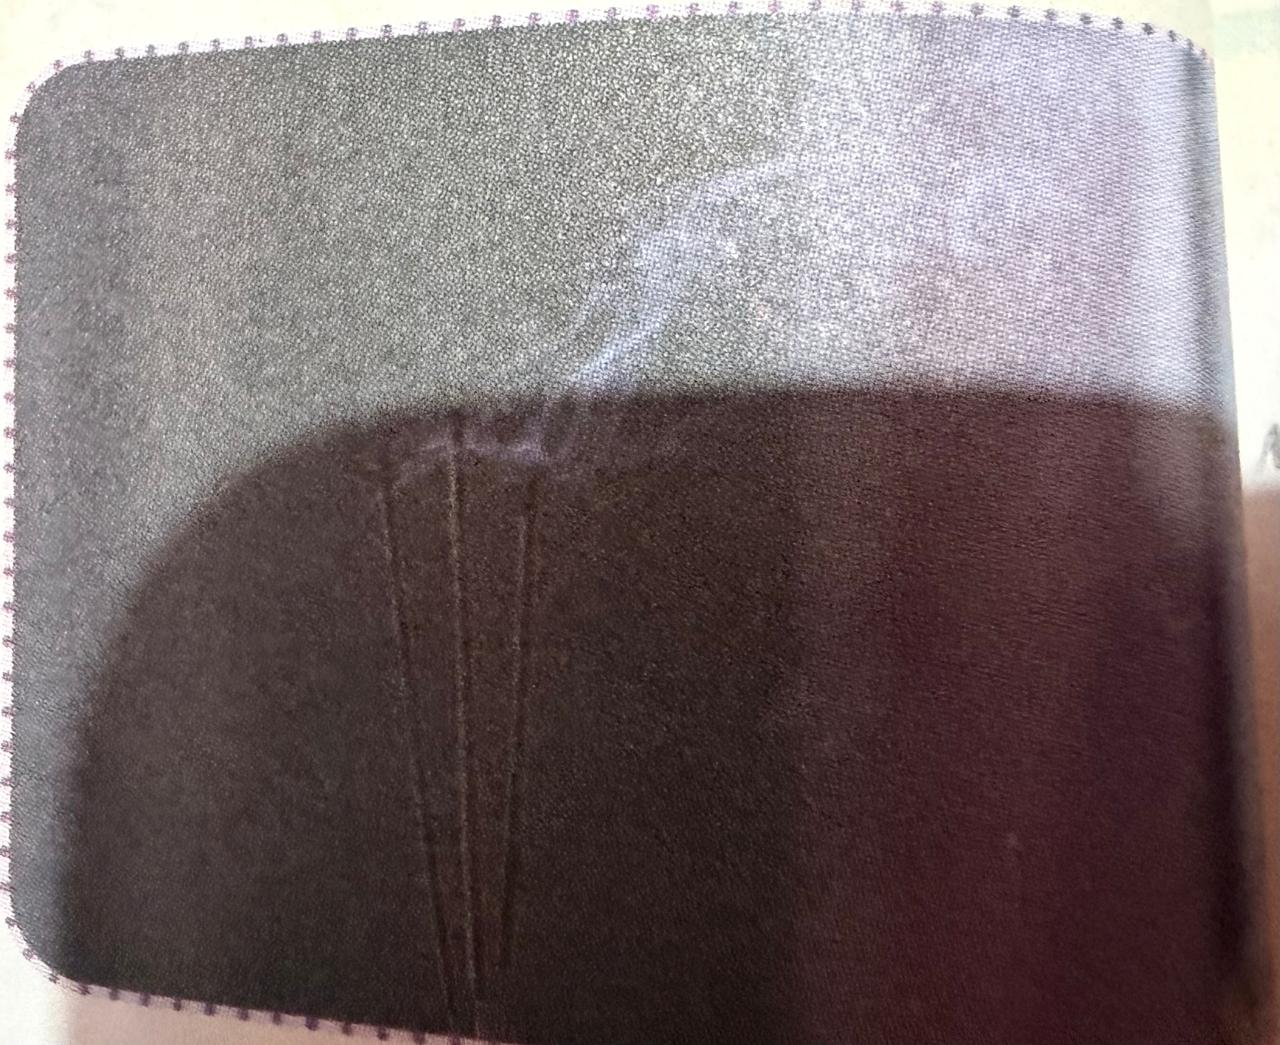
\includegraphics[width=0.5\linewidth]{../image/increasine_stick.jpeg}
    \caption{Gases with insence stick}
    \label{fig:my-stick}
\end{figure}
\subsection{\textbf{Particles of matter attract each other.}}
Try to break a piece of chalk. Now try breaking a piece of iron. What do you observe? You can break the chalk but not piece of iron. This is because the interparticle force attraction is very weak in the chalk but very strong on the piece of iron.
\section{\textcolor{red}{Solids}}\
In solids, the particles are closely packed. The force of attraction between the particles is very strong. The interparticle spaces are \textcolor{red}{negligible}.
\subsection{\textcolor{orange}{Properties of Solids}}
\begin{itemize}
    \item They have a fixed shape and a fixed volume.
    \item They cannot be compressed.
    \item They are rigid and do not flow.
\end{itemize}
\begin{figure}
    \centering
    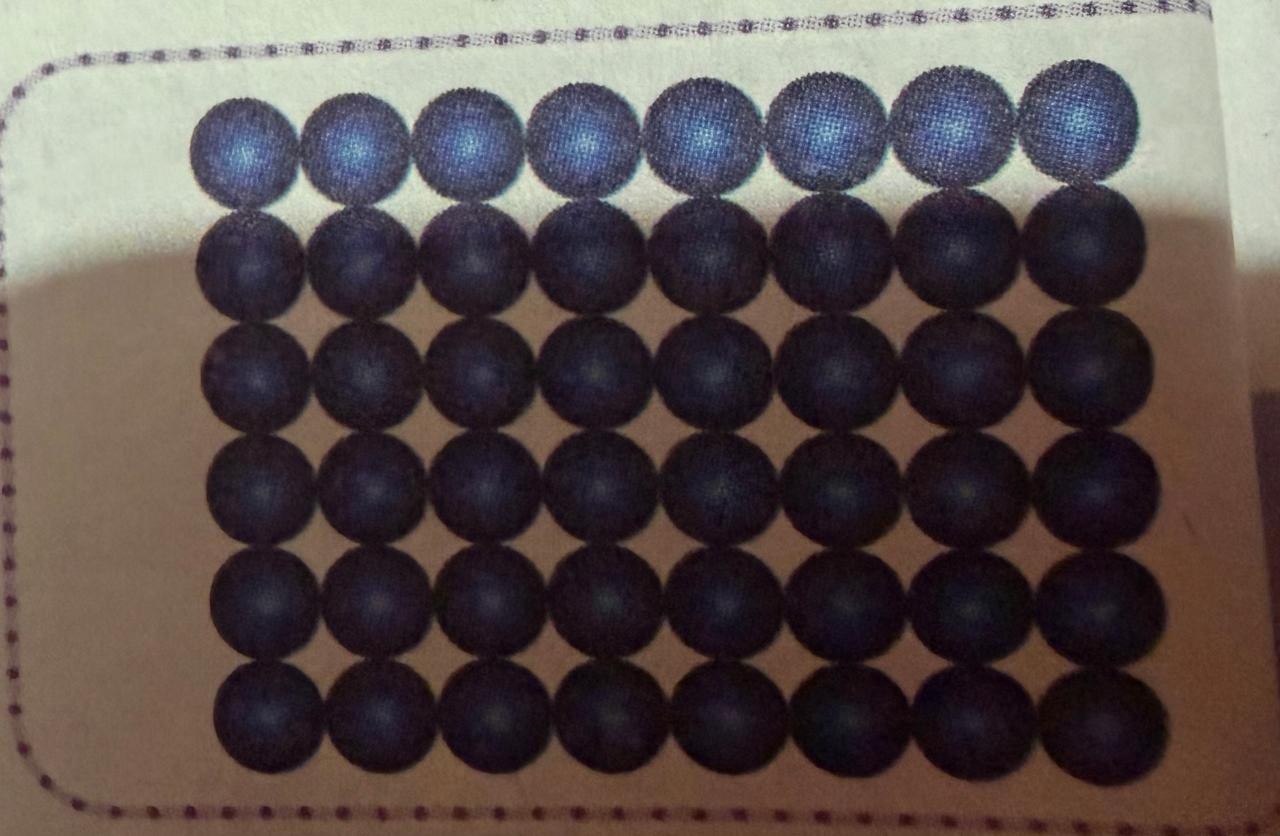
\includegraphics[width=0.5\linewidth]{image/solids.jpeg}
    \caption{Particles are too closer with solids}
    \label{fig:solid}
\end{figure}
\section{\textcolor{red}{Liquids}}
In liquids, the particles are not as closely packed as in solids. The forces of attraction in liquids are weaker than those in solids but stronger than those in gases.
\subsection{\textcolor{orange}{Properties of Liquids}}
\begin{itemize}
    \item Liquids do not have a fixed shape. They take shape of the container.
    \item They have a fixed volume.
    \item They cannot compressed much.
    \item They flow easily and are also known as fluids.
\end{itemize}
\begin{figure}
    \centering
    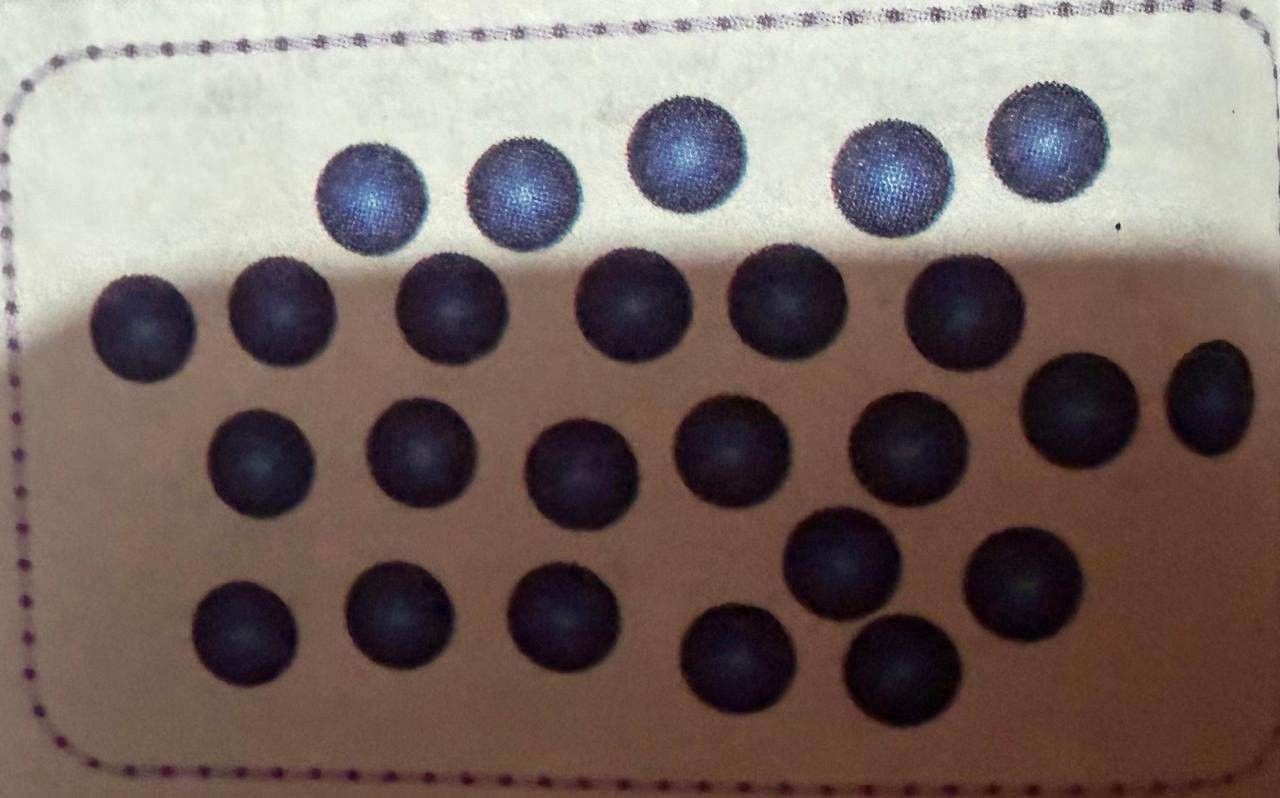
\includegraphics[width=0.5\linewidth]{../image/liquids.jpeg}
    \caption{Liquids the particles are volume}
    \label{fig:liquid}
\end{figure}
\section{\textcolor{red}{Gases}}
Gases, the particles are very far apart from the one another. The force of attraction between the particles is very weak.
\subsection{\textcolor{orange}{Properties of Gases}}
\begin{itemize}
    \item Gases have neither a fixed shape nor a fixed volume. They take the shape and the volume of the container.
    \item They can be compressed easily.
    \item They flow easily and are also known as fluids.
\end{itemize}
\begin{figure}
    \centering
    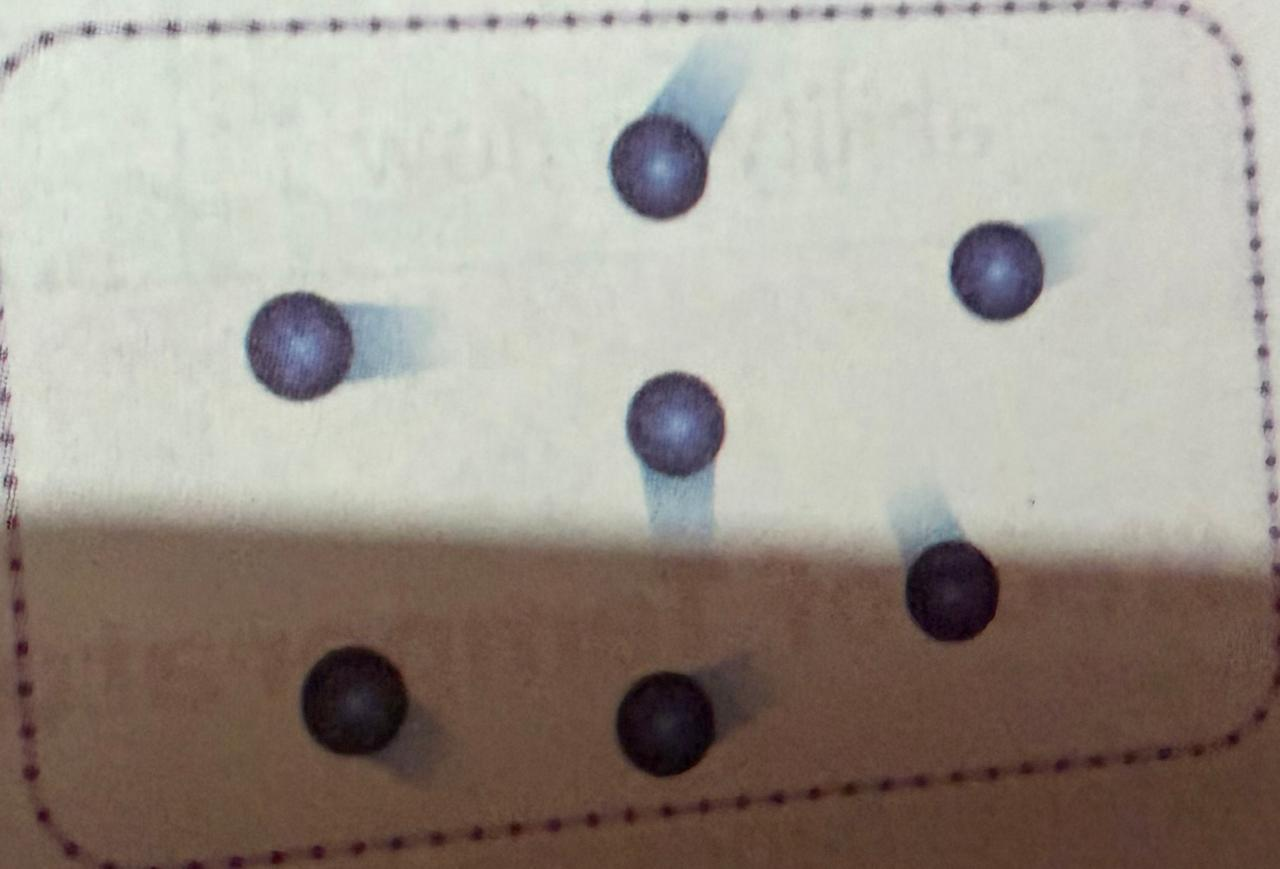
\includegraphics[width=0.5\linewidth]{../image/gases.jpeg}
    \caption{Particles are tooo far apart form one another}
    \label{fig:gas}
\end{figure}
\section{\textcolor{red}{Effect of Temperature on Matter}}
Matter expands on heating. Expansion can be seen in all the three states. On increasing the temperature, the intermolecular distance between particles of matter increases. This increase in distance causes expansion. After a particular stage, the energy of particles increases so much that they can overcome the force of attraction. This causes a change this state of matter.
\subsection{\textcolor{orange}{Expansion of Solids on Heating}}
Solids expand on heating. Electrical wires sag and railway tracks buckle in summers due to expansion.\begin{figure}
    \centering
    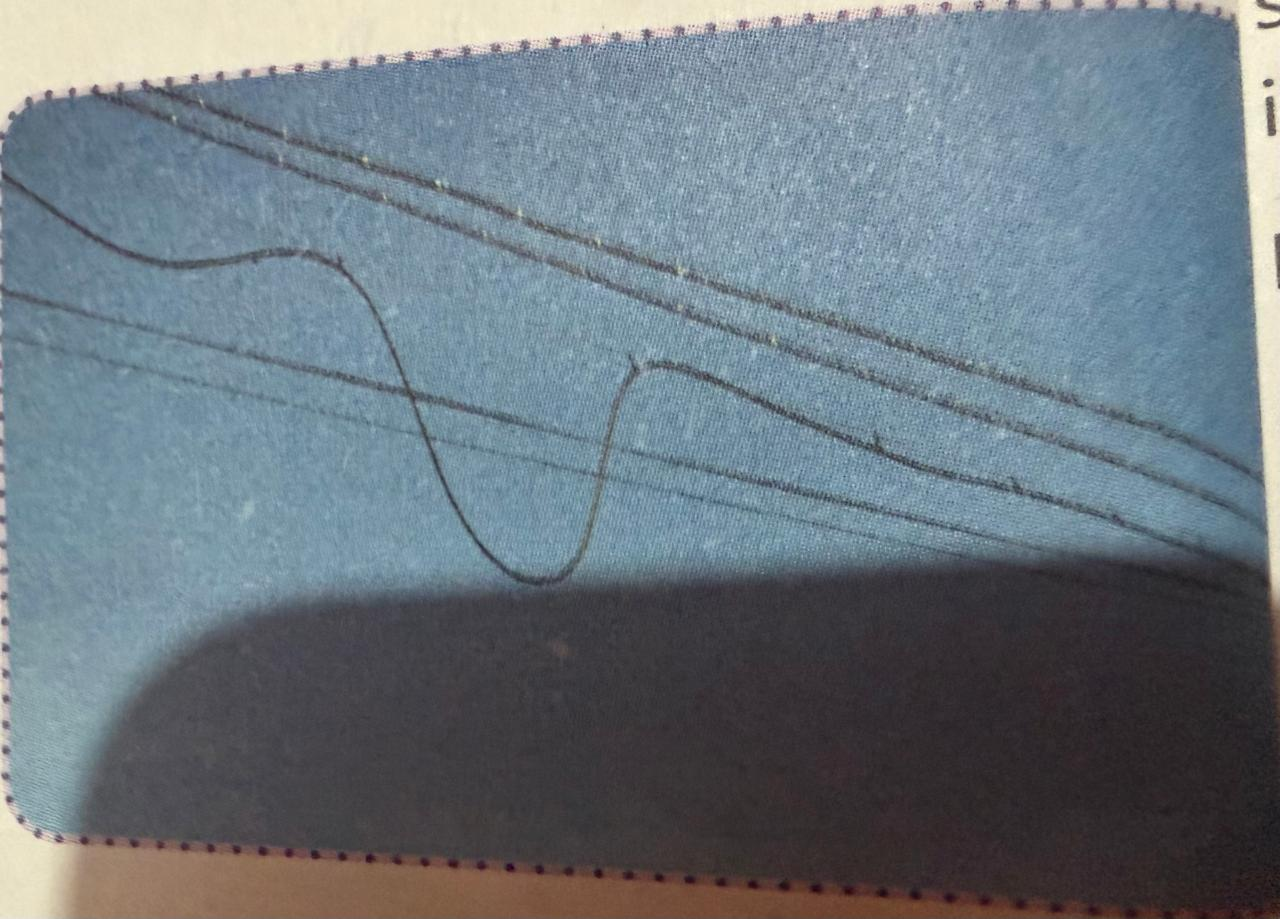
\includegraphics[width=0.5\linewidth]{../image/wires_sag.jpeg}
    \caption{When the summer due to expansion}
    \label{fig:wires}
\end{figure}
\subsection{\textcolor{orange}{Expansion of Liquids on Heating}}
Liquids also expand on heating. Let us see how liquids expand with the help of an example.\\
\par
 We use thermometer to check our body temperature. The thermometer has mercury in a thin tube inside it. When we put a thermometer in our mouth, the mercury inside the thin tube expands and rises due to body heat. We determine the temperature by reading the mark up to which the mercury has expanded.
 \subsection{\textcolor{orange}{Expansion of Gases on Heating}}
 Just like liquids, gases also expand on heating. You can observe this by covering the mouth of a bottle with a balloon. When the bottle is placed in hot water, the air inside the bottle expands and the ballon gets inflated.
 \begin{figure}
     \centering
     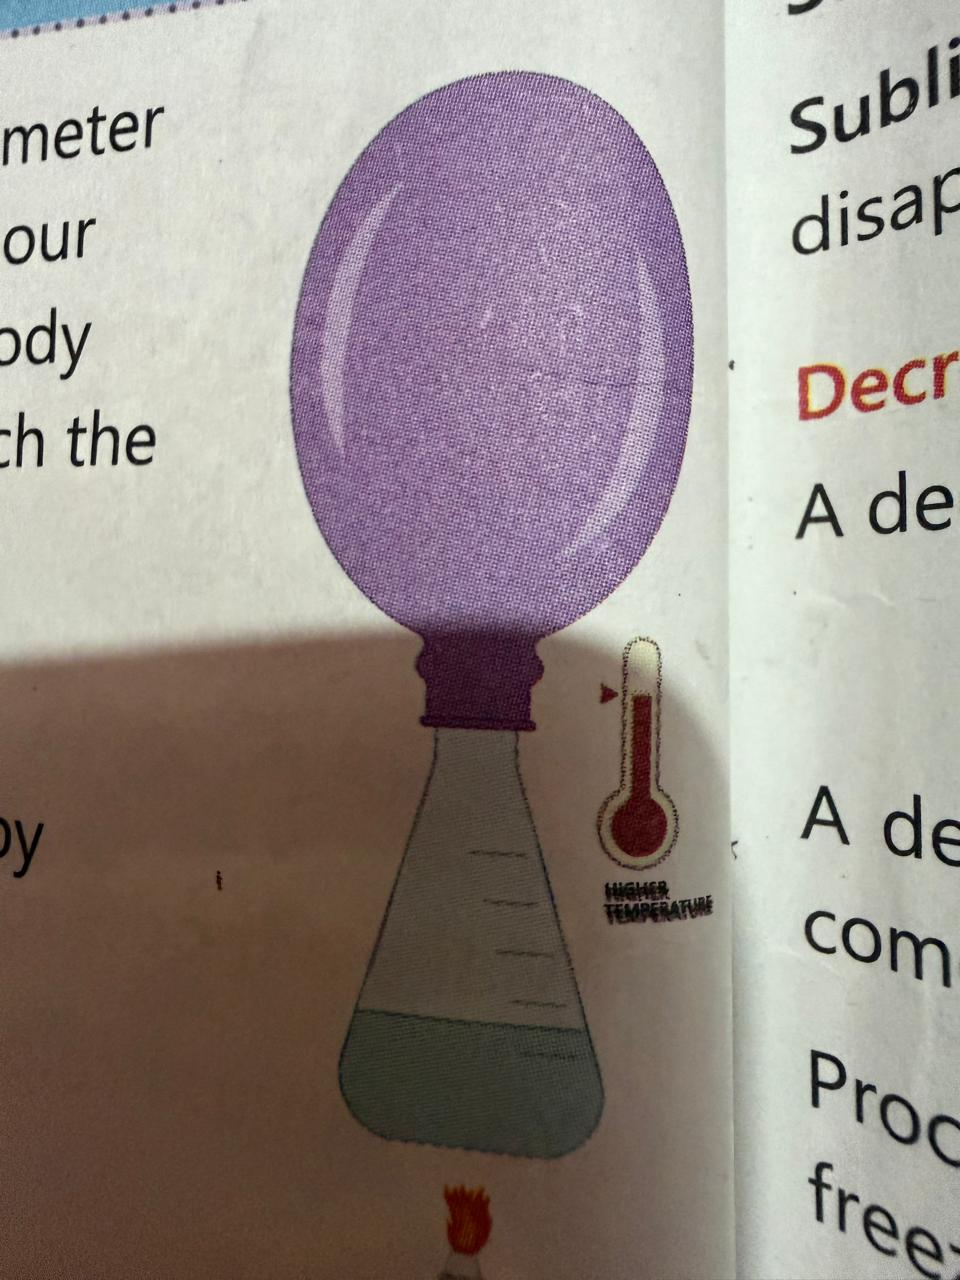
\includegraphics[width=0.5\linewidth]{../image/gases_with_ballon.jpeg}
     \caption{Ballon gets inflated}
     \label{fig:gases}
 \end{figure}
 \section{\textcolor{red}{Interconversion of States of Matter}}
 \textbf{Interconversion} is the change in the state of matter from the solid to liquid or liquid to gas or vice versa. We know that the particles of matter are continuous motion. By increasing or decreasing temperature, the energy with which the particles move increases or decreases. Thus, the  intermolecular force of attraction also changes. This causes matter to change its state.
\subsection{\textcolor{orange}{Increase in Temperature}}
An increase in temperature causes a conversion in the states of matter as follows:\\
\par
Solids $\rightarrow$ Liquids $\rightarrow$ Gases\\
\par
An increase in temperature increases the energy of the moving particles. Moreover, the energy supplied by heat also helps the particles to overcome the interparticle force of attraction.\\
\par
Process that take place due to an increase in temperature are melting, evaporation and sublimation.
\subsection{\textbf{Melting}} 
\textbf{Melting} is a process that involves reconversion of solids into liquids. For example ice, ice turns into a liquid.
\subsection{\textbf{Evaporation}}
\textbf{Evaporation} is the process of conversion of liquids into vapours. This process is involved in drying clothes in the Sun.
\subsection{\textbf{Sublimation}}
\textbf{Sublimation} is the process of conversion of solids into gases.  For example, gradual disappearance of naphthalene balls in the air.
\subsection{\textcolor{orange}{Decrease in Temperature}}
A decrease in temperature causes a conversion of the states of matter as follows:\\
\par
Gases $\rightarrow$ Liquids $\rightarrow$ Solids\\
\par
A decrease in temperature decreases the energy of particles and the particles of manner come close to each other.\\
\par
Processing that take place due to a decrease in temperature include condensation and freezing.
\subsection{\textbf{Condensation}} 
\textbf{Condensation} is the conversion of gases into liquids. For example, it is seen as formation water droplets on a glass containing a cold drink.
\subsection{\textbf{Freezing}}
It is the conversation of liquids into solids. For example, water changes into ice when place is in a freezer.
\begin{figure}
    \centering
    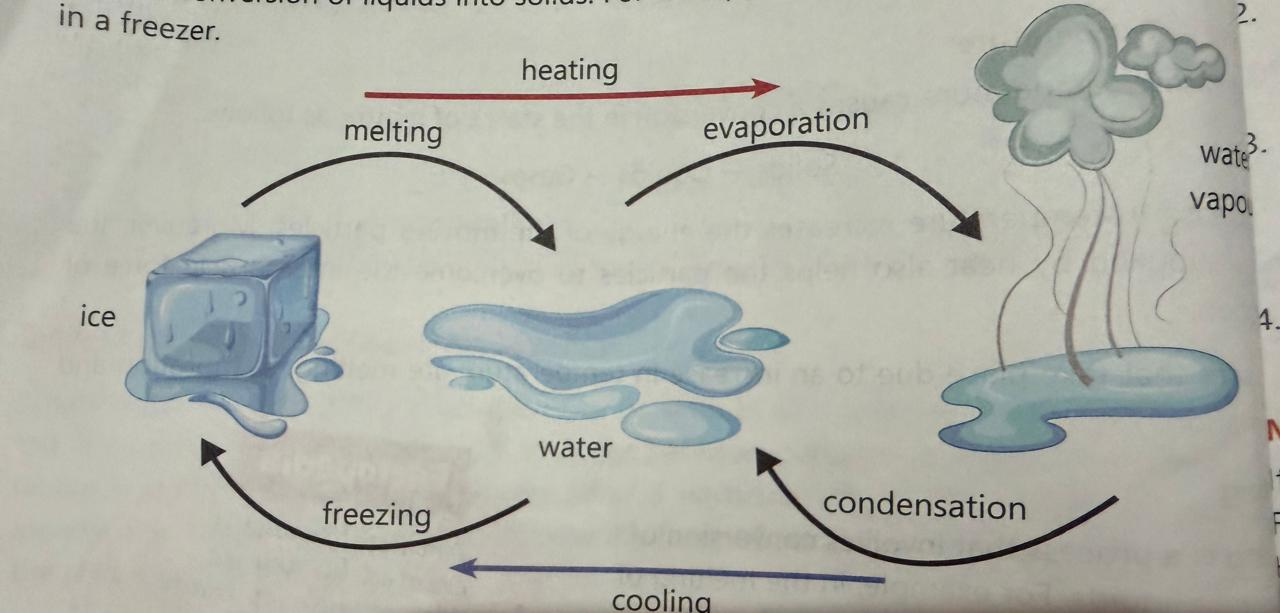
\includegraphics[width=0.5\linewidth]{image/Increase_decrease_temperature.jpeg}
    \caption{Heating and Cooling}
    \label{fig:temp}
\end{figure}
\section{\textcolor{red}{Solutions}}
A \textbf{solution} is like a special mixture. It is formed when two substances are mixed in a way that they are evenly distributed. A solution consists consists of two components - a solute and solvent.\\
\par
The \textbf{solvent} is the substance in which another substance in which another substance dissolves. The substance that gets dissolved in the solvent is the \textbf{solute.} For example, in a sugar solution, sugar is the solute and water is solvent.\\
\par
As many substances dissolve in water, it is known as the \textbf{universal solvent.}
\begin{figure}
    \centering
    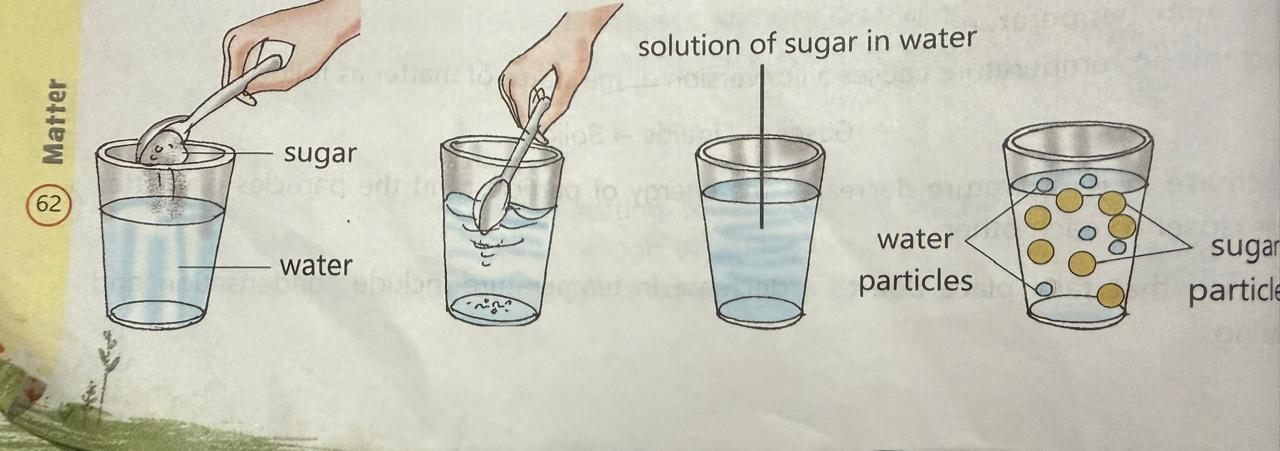
\includegraphics[width=0.5\linewidth]{../image/solution.jpeg}
    \caption{Water Particles and Sugar particles}
    \label{fig:solution}
\end{figure}
\subsection{\textcolor{orange}{Types of Solutions}}
Depending on the state of the solute and their solvent, solutions are classified into the following categories.
1. \textbf{Solid - it - liquid solutions:} These are formed when the solute is in the solid state and the solvent is in the liquid state. For example, a sugaara solution and a salt pollution.\\
2. \textbf{Liquid - in -liquid solutions:} These are formed when both the solute and the solvent are in the liquid state. For example, milk in water and lemon juice in water.\\
3. \textbf{Gas - in - liquid solutions:} These are found when the solute is in the gaseous state and the solvent is in the liquid state. For example, aerated drinks (carbon dioxide is dissolved in water) and oxygen dissolved in water.\\
4. \textbf{Gas - in - gas solutions:} These are formed when both the solute and the solvent are in the gaseous state. For example, air is mixture of different gases.\\
\par
\textcolor{red}{I wonder} if the volume of water increases when sugar is mixed into it!
\subsection{\textcolor{orange}{Miscrible and Immiscrible Liquids}}
If two liquids dissolve in each other when they are mixed, they are called \textcolor{red}{miscrible} \textbf{liquids.}
For example, when we make lemonade, lemon juice and water fully dissolve in each other. Here, lemon juice and water are \textbf{miscrible liquids.}\\
\par
On the other hand, if two liquids do not mix completely even if we try hard to mix them, they are called \textbf{immiscrible liquids.} These liquids from two separate layers. For example, if we keep an oil - water mixture undisturbed for some time, we can observe a layer of oil above water.
\begin{itemize}
    \item \textbf{Matter} is anything that occupies space and has mass.
    \item Solids, liquids and gases are the three \textbf{states of matter.}
    \item Matter is made up for small particles.
    \item Particles of matter have interparticle spaces between them. The particles keep moving and have forces of attraction between them.
    \item When matter is heated, it either expands or undergoes a change in state.\\
\end{itemize}